\chapter{Coexistence de bibliothèques dynamiques}
\label{ch:module_systems}


Ce chapitre traite du fonctionnement de l'éditeur de liens du système
d'exploitation (\textit{dynamique linker}) et des bibliothèques dynamiques. Le
système de modules, présenté dans ce mémoire, supporte le chargement de
plusieurs versions d'un module. Une version d'un module correspond à un
état de son code à un moment précis dans son évolution.
Cela a le potentiel de causer des problèmes d'exécution du programme. Puisque
ce système de module utilise des bibliothèques dynamiques du système
d'exploitation, il est donc nécessaire de déterminer la nature de ces
situations problématiques. Nous avons procédé à des expériences pour déterminer
sous quelles conditions des bibliothèques dynamiques peuvent coexister.

\section{Format des modules}

% Une bibliothèque de code est le regroupement de plusieurs types de données, des
% entiers, des nombres à virgule flottant, des chaînes de caractères, des
% fonctions et des données composites. L'ensemble de ces données constitue les
% fonctionnalités de la bibliothèque.

% Les fonctionnalités d'une bibliothèque peut être copié dans l'exécutable
% (bibliothèque statique), cela facilité la déploiement puisque que ses
% dépendances sont inclus dans un seul fichier.
La modularisation est utile pour séparer un programme en plusieurs composantes
relativement indépendantes. Ici nous traitons des modules au niveau du système
d'exploitation (``system libraries''). La forme dans laquelle un module est
stocké dépend du contexte. Dans les langages interprétés, les modules ont la
forme de fichier textuel, contenant du code, qui est compréhensible par un
humain. Cela facilite les modifications du code du module. Par contre,
l'interprétation de module en format textuel est beaucoup plus lente. Les
modules compilés sont l'alternative aux modules textuels.

Un module qui est compilé en format binaire est plus difficile à comprendre
du point de vue d'un humain, mais est plus rapide à s'exécuter. Le compromis
est la rapidité contre la lisibilité. Le format binaire peut varier d'un système
à l'autre. Les systèmes Linux utilisent le format ELF (\textit{Extensible Linking
Format}), Microsoft Windows le format PE (\textit{Portable Executable})
et macOS le format Mach-O (\textit{Mach object}). Ces formats binaires sont
utilisés pour les exécutables, les bibliothèques statiques et les bibliothèques
dynamiques.

Les bibliothèques dynamiques ont des problèmes propres comparativement aux
bibliothèques statiques.

% XXX: bytecodes aussi pour les langage compilé. (or ignore)

%Les langages
%de programmation interprétés fournisse leurs bibliothèques directement
%en code source. Dans cette catégorie, il y a Ruby, Python, Perl, Lua et
%Scheme -- dont le code des bibliothèques est écrit et frounit dans le
%langage respectif. Les langages compilés -- comme C, C++, C\# et Java --
%utilisent plutôt des formats binaires destiné, soit à une machine virtuelle
%(e.g. la \textit{Java Virtual Machine} JVM ou un architecture
%physique (e.g. i686, x86\_64, ARM). Les bibliothèques natives peuvent
%être utilisé


\section{Édition de liens dynamique}

une application qui utilise une bibliothèque partagée ne contient pas le code
de la bibliothèque, mais plutôt le nom des bibliothèques utilisées. la
récupèration le code à partir du nom est la résolution qui est effectuée par le
\textit{dynamic loader}.  lorsqu'un programme lié dynamiquement à plusieurs
bibliothèques partagées exécute un appel à une procédure externe, la routine de
résolution est démarrée pour résoudre le code de cette procédure.

%% bibiothèque dynamique native.
Par exemple, sous Linux l'utilitaire <<yes>>, qui est écrit en C,
est lié aux bibliothèques système suivantes:
\begin{verbatim}
  linux-vdso.so.1 (0x00007ffeef7f9000)
  libc.so.6 => /usr/lib/libc.so.6 (0x00007ff68161c000)
  /lib64/ld-linux-x86-64.so.2 => ...
\end{verbatim}

La bibliothèque \textit{libc.so.6} contient un grand nombre des fonctions
standards du système telles que \lstcode{fopen}, \lstcode{fclose},
\dots.  Le chargement de certaines bibliothèques utilisé par le \textit{dynamic
loader} est effectué au début de l'application, avant l'exécution de la fonction
principale souvent nommée \textbf{main}.  Plusieurs bibliothèques peuvent
coexister simultanément au sein d'un même processus sans que l'exécution du
programme en soit affectée.

La résolution des fonctionnalités de ces bibliothèques est effectuée par un
programme appelé le \textit{program interpreter} du système qui correspond à
\textit{/lib64/ld-linux-x86-64.so.2}.  Il est aussi possible de forcer la
résolution d'une fonctionnalité d'une bibliothèque de façon manuelle. Ce genre
d'interaction est possible sur les trois principales plateformes utilisées sur
le marché (Windows, macOS et Linux).

Sur Linux, l'API qui permet d'interagir avec les bibliothèques partagées provient de \textit{libdl.so}.
Elle contient les fonctions \textit{dlopen}, \textit{dlsym}, \textit{dlerror} et \textit{dlclose} pour gérer
des bibliothèques de code supplémentaire chargé manuellement à l'exécution.  Pour charger la fonction
\textit{foo}, qui ne prend pas d'argument et ne retourne rien de la bibliothèque \textit{libFoo.so} en C,
il faut exécuter les deux appels de la figure~\ref{fig:dlsym_dlopen}:
\begin{figure}[ht]
  \centering
\begin{lstlisting}[language=C,frame=single]
  ...
  void *handle = dlopen("./libFoo.so", RTLD_LAZY);
  void (*foo)() = dlsym(handle, "foo");
  ...
\end{lstlisting}
  \caption{Chargement dynamique de la bibliothèque \textit{libFoo.so} et
    résolution de la fonction \textit{foo} sans gestion d'erreur sous Linux}
    \label{fig:dlsym_dlopen}
\end{figure}\\
L'équivalent des bibliothèques partagées sous Windows est les DLLs, qui peuvent
être chargées de façon similaire dans un programme en utilisant les fonctions
\textit{LoadLibrary}, \textit{LoadLibraryEx} et \textit{GetProcAddress}. Ils
fonctionnent de la même façon que leur équivalent Linux. Pour macOS, il faut
passer par les routines:
\begin{itemize}
    \item \textit{NSCreateObjectFileImageFromFile}
    \item \textit{NSLinkModule}
    \item \textit{NSLookupSymbolInModule}
    \item \textit{NSAddressOfSymbol}
\end{itemize}

La majorité des langages interprétés permettent l'importation de bibliothèques
de code natives, via une interface nommée \textit{foreign function interface}
(FFI).  Cette interface offre une couche d'abstraction de ces procédures.
Prenons comme exemple les langages Python, Ruby, Lua et Scheme. Python possède
le module \textbf{ctypes} qui permet de charger des bibliothèques natives
dynamiques, et Ruby possède le module \textbf{ffi}.
%Ces modules ne font qu'encapsuler les fonction de chargement de bibliotheques
%native pour qu'il puisse être invoqué dans le langage cible.

% Bibliothèque Lua en C
% - La bibliothèque doit avoir le même nom que celui utilisé par le \textit{import}.

Certains langages ont un mécanisme pour charger des bibliothèques natives s'ils
ont été conçus spécialement.  Dans le langage de programmation Lua, il est
possible de charger directement une bibliothèque dynamique si elle contient une
fonction \textbf{luaopen\_\textit{libname}} où \textit{libname} est le nom de
la bibliothèque.  Gambit Scheme utilise un mécanisme équivalent. Il permet le
chargement de ces modules qui ont été compilés en bibliothèque partagée (DLL)
avec la fonction \texttt{(\textbf{load} "libname")}.

%% Python
%\begin{figure}[ht]
%\begin{lstlisting}[language=python,frame=single]
%# From https://docs.python.org/2/library/ctypes.html
%from ctypes import *
%# Chargement d'une bibliotheque native.
%lib = cdll.LoadLibrary("./libFoo.so")
%# Appel de la fonction foo.
%lib.foo()
%\end{lstlisting}
%\caption{Code d'importation de la fonction \textbf{foo} de la bibliothèque \textit{libFoo.so} en Python}
%\end{figure}

\begin{center}
% Ruby
\begin{figure}[ht]
\begin{lstlisting}[language=ruby,frame=single]
require 'ffi'
# Chargement d'une bibliotheque native.
module LibFoo
    extend FFI::Library
    ffi_lib './libFoo.so'
    attach_function :foo, [], :void
end
# Appel de la fonction foo.
LibFoo.foo
\end{lstlisting}
\caption{Code d'importation de la fonction \textbf{foo} de la bibliothèque
  \textit{libFoo.so} en Ruby}
\end{figure}
\end{center}

La résolution des fonctionnalités effectuée par le \textit{dynamic linker}
utilise un ordre de recherche défini. Cet ordre de recherche inclut
l'exécutable courant, les dépendances de l'exécutable, la bibliothèque passée à
\textit{dlsym}. Une résolution d'une fonctionnalité est soit directe ou
indirecte. La résolution d'une fonctionnalité par \textit{dlsym} qui n'engendre
pas la résolution d'une autre fonctionnalité externe est directe. Une résolution
directe n'utilise pas le programme principal dans l'ordre de recherche.
Les résolutions de fonctionnalité provenant d'appels indirects au
\textit{dynamic linker} inclut le programme principal et ses dépendances avant
la bibliothèque passée à \verb|dlsym|.

\begin{center}
    \begin{figure}[ht]
        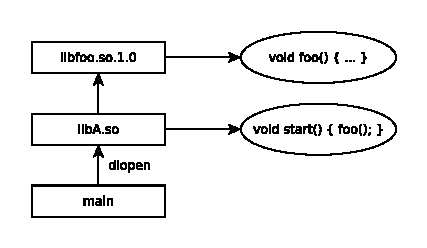
\includegraphics{figures/libdeps-ex1.pdf}

        \caption{Un exemple de dépendance de bibliothèques au sein d'une
          application simple fictive.  La bibliothèque \textit{libA.so} est
          chargée dans l'application \texttt{main} via les appels aux procédures
          \textit{dlopen} et \textit{dlsym}. Les fonctionnalités utilisées dans
          l'exemple sont marquées dans des ellipses.}

        \label{fig:deps-ex1}
    \end{figure}
\end{center}

Dans la situation présentée dans la figure~\ref{fig:deps-ex1}, quelles sont les
étapes incluses dans l'exécution de ce programme qui invoque la fonctionnalité
\texttt{start} de la bibliothèque \textit{libA.so}? La fonctionnalité externe
\texttt{start} est résolue de façon directe par un appel à
\verb|dlsym(libA,"start")| qui commence la recherche de la procédure
\texttt{start} dans la bibliothèque spécifiée en paramètre \texttt{dlsym}. Le
programme l'invoque une fois la procédure trouvée.  L'appel à une procédure non
résolue (e.g.\ la procédure \texttt{foo} invoquée dans \texttt{start})
déclenche une procédure automatique de résolution des fonctionnalités. Cette
procédure de résolution commence sa recherche à partir de l'exécutable, puis
itère la liste des dépendances directe. Si la fonctionnalité n'est pas encore
trouvée, la recherche continuera à partir de la bibliothèque passée à
\texttt{dlsym}.

% Stub

Il est facile d'exploiter l'ordre de recherche du \textit{dynamic linker} pour
causer un masquage de fonctionnalité dans une application. Ce masquage est
utilisé dans certains contextes pour déboguer un programme, mais il peut aussi
nuire à l'exécution du programme. Il y a au moins deux structures de programme
qui causent un masquage. L'application principale est construite comme une
bibliothèque dynamique exécutable et fournit une fonctionnalité qui porte le
même nom qu'une fonctionnalité exportée par une bibliothèque externe chargée
manuellement.  L'application principale est liée avec une bibliothèque qui
exporte une fonctionnalité qui porte le même nom que celle utilisée dans la
bibliothèque externe.

La figure~\ref{fig:deps-ex2} est un exemple de masquage qui utilise la seconde
méthode. La première méthode requiert des bibliothèques exécutables qui ne sont pas
disponibles sur toutes les plateformes. Sous Linux, il est possible de créer une
bibliothèque exécutable en passant le paramètre \texttt{-rdynamic} à \textit{gcc}
lors de la construction de la bibliothèque.

\begin{figure}[ht]
  \centering
  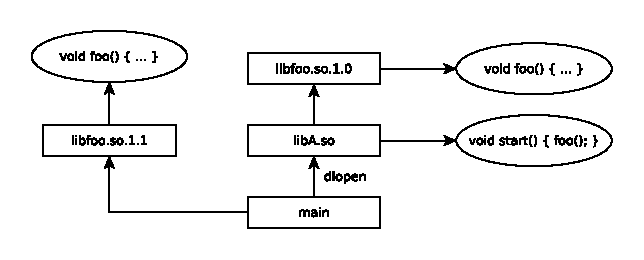
\includegraphics{figures/libdeps-ex2.pdf}
  \caption{Exemple de dépendance dans une application qui cause le masquage de
  la fonctionnalité \texttt{foo} de la bibliothèque \textit{libfoo.so.1.0} par
  la bibliothèque \textit{libfoo.so.1.1}}
  \label{fig:deps-ex2}
\end{figure}
%% BEGIN
% D'autre langage compilé comme C/C++
% ne le permette pas directement, la liste des bibliothèques de code utilisé par un
% programme est déterminée lors de la création du fichier binaire, qui peut être
% soit un exécutable où une bibliothèque.
%% END


% TODO: pourquoi est-ce utile?  XXX: structure pas final.
% - Les bibliothèques coexistent dans les application de tous les jours.
L'analyse des interactions entre des bibliothèques au sein d'un même programme
permet de mieux comprendre quelles sont les circonstances qui peuvent conduire
à des comportements non désirés, comme le masquage de fonctionnalité présent
dans l'exemple de la figure~\ref{fig:deps-ex2}.  Cela permet aussi d'établir
les conditions qui permettent d'éviter ces comportements non désirés.

\subsection{Coexistence entre les bibliothèques}

Les bibliothèques coexistent dans deux contextes principaux, de façon passive
dans un système de fichier et de façon active durant l'exécution d'un
programme.  Un système de fichier contient une arborescence hiérarchique de
répertoires et de fichiers avec une seule racine. Un fichier est l'entité dans
un système de fichier qui contient le code des bibliothèques.  Les répertoires
sont les entités qui permettent de regrouper plusieurs fichiers de façon logique.
La racine correspond au sommet de la hiérarchie du système de fichier. La façon
de référer à un fichier dans un système de fichier est d'utiliser le chemin
absolu. Cela correspond à la liste des répertoires à parcourir de la racine
jusqu'au fichier. L'outil responsable d'organiser les bibliothèques sur un
système est le \textit{package manager}. Il a plusieurs objectifs incluant
l'installation de bibliothèque, la mise à jour des bibliothèques installées, la
désinstallation de bibliothèque et la résolution des dépendances.

Un cas intéressant de coexistence entre bibliothèques est celui qui inclut
plusieurs versions d'une bibliothèque. Les problèmes peuvent être liés à
l'organisation sur le système de fichier et au masquage de fonctionnalité
durant l'exécution d'un processus.  Il y a aussi plusieurs utilités de
conserver plusieurs versions d'une bibliothèque, cela permet de supporter des
applications qui dépendent de bibliothèques antérieures.

Une autre application est de convertir un vieux format de fichier vers un
format plus récent. Dans le cas où il n'est pas possible d'avoir en même temps
plusieurs versions d'une bibliothèque, il faut alors écrire un parseur pour
lire le vieux format, ensuite utiliser les fonctions de la version cible de la
bibliothèque pour générer le nouveau format du fichier.  Cette solution est
clairement laborieuse et susceptible à des erreurs de codage.

\begin{figure}[ht]
  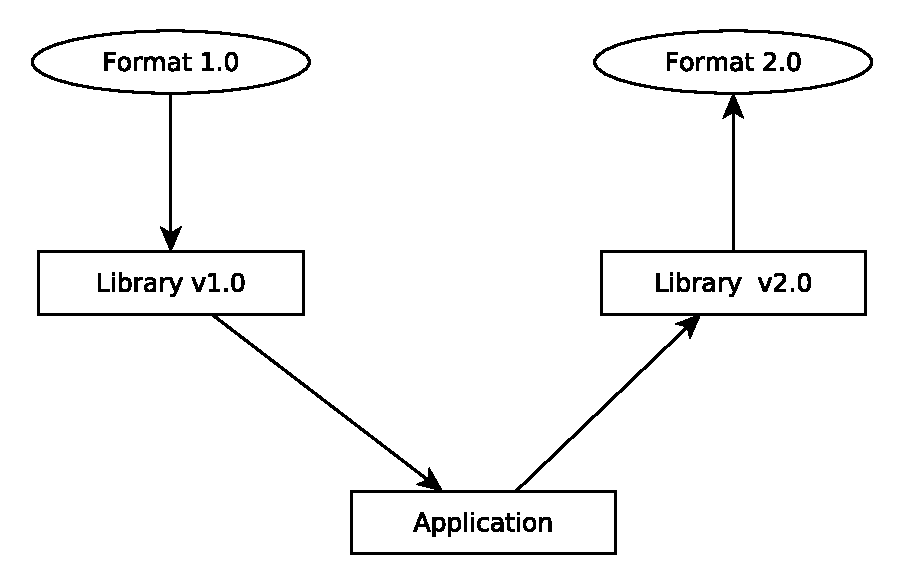
\includegraphics[width=30em]{figures/app_convert_v1_to_v2.pdf}
  \caption{Un exemple d'application de conversion entre deux versions d'un format
  de fichier comme sqlite2 et sqlite3 exploitant la possibilité de charger plusieurs
  versions d'une bibliothèque.}
\end{figure}

% L'architecture de processus sur un système permet plusieurs propriétés. La
% robustesse, un processus failli les autres processus ne sont pas affectés. La
% sécurité et l'isolation, chaque processus possède leur mémoire qui n'est pas
% accessible par les autre processus et peuvent utilisé une version spécifique
% des bibliothèques. Il est possible de concevoir l'architecture de processus en
% utilisant des threads.  Un \textit{thread} décrit un courant d'exécution d'un
% programme. Un processus à au minimum un \textit{thread} qui correspond au
% courant d'exécution principal du programme. Les \textit{threads} sont utiles
% pour paralléliser l'exécution d'un processus. La création de \textit{threads}
% est beaucoup plus rapide que la création d'un processus, car elle ne nécessite
% pas l'appel au système d'exploitation.

% Ce modèle exploite la légèreté des \textit{threads} par rapport au processus et
% la possibilité de charger plusieurs version des bibliothèques qu'il a besoin au sein
% du système. Cela est similaire au modèle de processus utilisé par les
% système d'exploitation, sauf que l'ensemble est juste au sein d'un seul processus.
% Étant donnée que les \textit{threads} vivent tous au sein d'un même processus,
% il est donc facile de partagé des informations d'un \textit{thread} à un autre.
% Ce qui est plus difficile avec le modèle de processus, cela nécessite l'utilisation
% mécanisme comme la mémoire partagé.

%et s'il c'est un cas qui peut
%contenir un coexistence néfaste.  Cela n'est possible que s'il est possible de
%distinguer les deux version de la bibliothèque et aussi répartir les appels à
%des fonctions de même nom à la bonne version de la bibliothèque.

\section{Conditions de coexistence}
%
Des conditions suffisantes pour que deux bibliothèques puissent coexister
au sein d'un processus incluant deux versions de la même bibliothèque
sont l'absence d'état global ou local, et l'unicité des noms des
fonctionnalités.  L'absence d'état garantit que chaque fonction de la
bibliothèque retourne toujours un résultat prévisible dans un contexte
identique. Un cas extrême est la pureté fonctionnelle, qui est d'autre part
avantageuse dans un contexte \textit{multithread}, car il n'est pas possible
d'avoir une condition de course sur une donnée partagée. La pureté
fonctionnelle garantit qu'il n'y a pas d'affectation et donc pas d'état.  Le
fait que chaque fonctionnalité soit associée à un nom unique qui empêche une
bibliothèque de masquer une fonctionnalité d'une autre bibliothèque.


% Une condition de courses survient lorsque l'ordre des opérations d'un programme
% s'exécute dans un ordre que le programmeur n'a pas conçu. Par exemple, un
% application avec deux fils d'exécutions, un qui lit la valeur d'une variable
% globales l'autre qui l'écrit.  Deux scénarios sont possible, la lecture peut
% s'effectuer avant ou après la la modification de la variable globale selon
% l'ordonnancement de ces deux fils d'exécution.  Le résultat de la lecture est
% dépendant de l'ordonnancement de ces deux opérations.

Ces conditions sont suffisantes pour que deux bibliothèques coexistent sans
problème, mais elles ne sont pas nécessaires. Il existe des bibliothèques qui
ne respectent pas ces conditions, mais coexistent avec d'autres versions de la
bibliothèque.  Pour tester la coexistence entre plusieurs bibliothèques, des
expériences ont été effectuées dans plusieurs systèmes de modules existants. Le
but de l'expérience est d'observer le bon fonctionnement des bibliothèques au
sein du processus.

Les expériences qui suivent permettent d'observer et d'identifier les cas de
cohabitation de bibliothèques au sein d'une application qui cause des
problèmes. Ils permettent aussi d'identifier les capacités d'un langage à
charger plusieurs versions d'une bibliothèque.

% XXX
%La capacité d'un langage d'interfacer avec d'autre langage via la FFI propage
%les limitations du langage cible.


\subsection{Bibliothèque C}
%
Les bibliothèques dans le langage C sont compilées dans un format natif pour la
plateforme courante (e.g. Window, macOS, Linux). Leur format diffère d'un
système d'exploitation à un autre, Window utilise le format \textit{dll}
(\textit{dynamic loading library}), macOS utilise le format \textit{dylib}
(\textit{Mach-O dynamic library}) et Linux utilise le format \textit{so}
(\textit{shared object}).

Les bibliothèques C consistent de symboles qui correspondent aux fonctions et
variables globales exportées. Une bibliothèque est généralement liée à un
programme C lors de la création du programme. Les symboles non définis sont
résolus durant l'exécution du programme.

% TODO: complete
% - Bibliotheques avec collisions de nom de symboles
% - Masquage de fonctionnalité d'une des deux bibliothèque
Les collisions de symboles entre deux bibliothèques causent un masquage de
fonctionnalité d'une des deux bibliothèques. Un problème est de savoir si cela
est possible de charger deux bibliothèques avec des collisions de symboles et
accéder aux fonctionnalités distinctes de ces bibliothèques.

Pour charger deux versions d'une même bibliothèque en C, il faut utiliser un
moyen qui prend en compte des symboles communs.  La résolution des symboles se
fait par un parcourt en largeur dans la liste des symboles des bibliothèques.
Le résultat est le premier objet qui correspond au nom de symbole recherché.
L'ordre des bibliothèques utilisé dans la résolution des symboles correspond à
l'ordre spécifié lors de la construction de l'exécutable.

%    \vspace{-10pt}
\begin{center}
\begin{figure}[ht]
\begin{lstlisting}[frame=single]
> gcc -lSDL -lSDL2 exemple.c -o exemple
> ldd ./exemple
libSDL.so => /usr/lib/libSDL.so
libSDL2.so => /usr/lib/libSDL2.so
\end{lstlisting}
\caption{Création d'un exécutable lié aux deux bibliothèques
SDL et SDL2 dans cet ordre.}
\label{fig:sdl_mask_sdl2}
\end{figure}
\end{center}

La figure \ref{fig:sdl_mask_sdl2} donne la procédure de création d'un
exécutable lié avec deux versions de SDL.  Les tests ont été effectués sur deux
versions de SDL, 1.2 et 2. Ces versions peuvent utiliser des ressources communes comme
les événements du clavier, la mémoire et le GPU en utilisant OpenGL pour faire
de l'affichage 2D ou 3D.  Plusieurs situations sont testées, chacune sans thread
et avec des threads:
%
\begin{enumerate}
    \item Une utilisation de SDL minimaliste qui n'écoute pas les événements utilisateurs.
    \item Une utilisation de SDL avec une boucle d'événements de base.
    \item Une utilisation de SDL avec une utilisation d'un contexte OpenGL.
\end{enumerate}

%% SDL1.2 appel ces propres fonctions et SDL2 appel ces propres fonctions.
Puisque SDL1.2 et SDL2 ont des collisions de symboles (e.g.\ \verb+SDL_Init+,
\verb+SDL_FillRect+, \verb+SDL_BlitSurface+, \dots), l'une des premières
observations à effectuer est la bonne répartition des appels de fonctions des
deux bibliothèques dans le contexte d'une même application. Le problème à
identifier est un appel invalide à une procédure de SDL2 qui était destiné à
SDL1.2. Le facteur, qui influence laquelle des deux bibliothèques va masquer
l'autre, est l'ordre dans laquelle elles sont liées au programme à la création,
qui est montrée à la figure~\ref{fig:sdl_mask_sdl2}.

Le masquage est un problème qui peut mener à une défaillance du
programme, car cela peut provoquer la transmission d'une structure incompatible
de la première bibliothèque à la deuxième. Dans le cas de SDL, la structure
\verb+SDL_Surface+ à une disposition différente des champs, donc incompatible.
Le premier champ qui décale l'alignement de ces deux structures est le
\textit{pitch}, qui dans SDL1.2 est déclaré en Uint16 alors qu'en SDL2 il est
un int qui sont des types de taille différente. Donc, l'accès au prochain champ
\texttt{pixels} est différent entre SDL1.2 et SDL2, ce qui peut causer un accès
invalide en mémoire. si une structure de SDL1.2 est accédée comme une structure
de SDL2.

% XXX: ANTIDOTE_MARKER

\begin{figure}[h]
  \centering
\begin{tabular}{p{18em}p{18em}}
\begin{lstlisting}[frame=single,numbers=left]
typedef struct SDL_Surface {
    Uint32 flags;
    SDL_PixelFormat *format;
    int w, h;
    Uint16 pitch;
    // Different offset here
    void *pixels;
    ...
} SDL_Surface;
\end{lstlisting}&
\begin{lstlisting}[frame=single,numbers=right]
typedef struct SDL_Surface {
    Uint32 flags;
    SDL_PixelFormat *format;
    int w, h;
    int pitch;
    // Different offset here
    void *pixels;
    ...
} SDL_Surface;
\end{lstlisting}\\
\end{tabular}
  \caption{La comparaison entre la structure \textbf{SDL\_Surface} de SDL1.2 et SDL2 respectivement.}
  \label{fig:sdl_surface}
\end{figure}

%% Instable: gcc -lSDL -lSDL2 ...
%Puisque les programmeurs cherchent une certaine stabilité dans leurs bibliothèques, ils ont
%tendance à éviter les dépendances avec des bibliothèques qui ont des collisions de fonctionnalités.

La coexitence entre deux bibliothèques conflictuelles au sein d'une application
n'est pas possible en lien l'application aux bibliothèques durant sa
construction~\ref{fig:sdl_mask_sdl2}.  Il est peu probable d'avoir une
coexistance entre deux bibliothèques avec des noms de fonctionnalités
similaires au sein.

La façon d'avoir plusieurs bibliothèques conflictuelles au sein d'un programme
est d'utiliser l'API du \texttt{dynamic linker}.  Le cas qui pourrait permettre
plusieurs bibliothèques avec des collisions de symboles au sein d'une même est
avec l'API du \textit{dynamic linker}. Un test simple permet de démontrer la
capacité de répartir les appels d'une fonction identifiés par le même nom dans
différentes bibliothèques.

La structure générale des tests est organisée comme suit. Deux bibliothèques implémentant
une interaction valide avec l'une des versions de la bibliothèque (e.g. SDL1.2, SDL2).
Une application qui unit ces deux bibliothèques en utilisant l'API du
\textit{dynamic linker} pour exécuter ces deux bibliothèques séquentiellement ou
parallèlement.

%% TODO: expliquer la structure des programmes.

Dans le test minimaliste sans gestion d'évènements, l'exécution des bibliothèques
fonctionne dans les deux cas, séquentiellement et en parallèle. La raison qui
explique ce bon fonctionnement est la répartition des appels aux fonctions
des deux bibliothèques et le fait qu'il n'utilise pas de structure commune,
qui pourrait causer des conditions de course dans le test en parallèle.

\begin{center}
  \begin{figure}[ht]
\begin{lstlisting}[language=C,frame=single]
#include <SDL/SDL.h>

int main(int argc, char **argv) {
  SDL_Init(SDL_INIT_VIDEO);
  SDL_WM_SetCaption("sdl1_2", NULL);
  SDL_Surface *win =
    SDL_SetVideoMode(200, 200, 24, SDL_HWSURFACE);

  Uint32 color = SDL_MapRGB(win->format, 255, 0, 0);

  SDL_FillRect(win, NULL, color);
  SDL_Flip(win);
  SDL_Delay(1000);

  SDL_FreeSurface(win);
  SDL_Quit();
  return 0;
}
\end{lstlisting}
    \caption{Programme qui utilise la bibliothèque SDL1.2 sans la gestion des évènements
    Cette application génère une fenêtre rouge qui se ferme après 1 seconde de délais.}
  \end{figure}
\end{center}

%TODO: wrap these into frame
\begin{center}
  \begin{figure}[ht]
\begin{lstlisting}[language=C,frame=single]
#include <SDL2/SDL.h>

int main(int argc, char **argv) {
  SDL_Init(SDL_INIT_VIDEO);
  SDL_Window *win = SDL_CreateWindow("title",
      SDL_WINDOWPOS_CENTERED, SDL_WINDOWPOS_CENTERED,
      200, 200, SDL_WINDOW_SHOWN);
  SDL_Surface *screen = SDL_GetWindowSurface(win);

  Uint32 color = SDL_MapRGB(screen->format, 0, 255, 0);
  SDL_FillRect(screen, NULL, color);
  SDL_UpdateWindowSurface(win);
  SDL_Delay(1000);
  SDL_DestroyWindow(win);
  SDL_Quit();
  return 0;
}
\end{lstlisting}
    \caption{Programme qui utilise la bibliothèque SDL2 sans la gestion des évènements.
    Cette application génère une fenêtre verte qui se ferme aussi après 1 seconde de délais.}
  \end{figure}
\end{center}

Dans le test incluant des évènements, l'hypothèse supposait que les évènements du clavier
auraient causé des problèmes de conditions de course en parallèle. Le test a aussi fonctionné
séquentiellement et en parallèle, malgré la dépendance commune du clavier.

Le test qui incluait OpenGL, n'aurait pas dû fonctionner par hypothèse. Les deux versions
de SDL référaient à une unique version de OpenGL. Le résultat a été surprenant, car le test
séquentiel et parallèle à fonctionné. Ce qui amène à conclure qu'il existe des cas
de coexistence entre des bibliothèques avec des collisions de symbole qui fonctionne
sans causer des problèmes d'exécution.



%%% Possible de compile le programme principale en un exécutable et en bibliothèque.
%Les deux programmes sont compilés en bibliothèques et en exécutables.
%Le fonctionnement de chaque programme est testé de façon séparé.
%Le programme principale, qui charge le main des deux autres programmes en utilisant
%l'API du \textit{dynamic loader}, est compilé en mode séquentiel et en mode parallèle.
%La version séquentielle permet d'observer la coexistance entre les deux bibliothèques,
%celle parallèle est utilisé pour évaluer les conditions de course sur des ressources
%communes.
%
%%% TODO: schema.
%\begin{center}
%  \begin{figure}[ht]
%\begin{lstlisting}[language=C,frame=single]
%  ...
%  void *hndl1 = dlopen(prog1, RTLD_NOW);
%  void *hndl2 = dlopen(prog2, RTLD_NOW);
%
%  int(*main1)(int,char**) = dlsym(hndl1, "main");
%  int(*main2)(int,char**) = dlsym(hndl2, "main");
%
%  main1(argc, argv);
%  main2(argc, argv);
%  ...
%\end{lstlisting}
%  \caption{Le chargement et exécution séquentiel de la fonction main des programmes
%  \textbf{prog1} et \textbf{prog2} via l'API du \textit{dynamic loader}.}
%  \end{figure}
%\end{center}
%% \begin{center}
%%   \begin{figure}[ht]
%% \begin{lstlisting}[language=C,frame=single]
%% struct MainCallback {
%%   int argc;
%%   char **argv;
%%   int (*main)(int,char**);
%% };
%%
%% void *run(void* args) {
%%   struct MainCallback* callback = (MainCallback*)args;
%%   callback->main(callback->argc, callback->argv);
%%   return NULL;
%% }
%% \end{lstlisting}
%%   \caption{Callback utilisé pour exécuté le main de la bibliothèque chargé par
%%   \textbf{dlsym} en parallèle avec pthread.}
%%   \end{figure}
%% \end{center}
%
%\begin{center}
%  \begin{figure}[ht]
%\begin{lstlisting}[language=C,frame=single]
%  ...
%  struct MainCallback callback = {
%    .argc = argc,
%    .argv = argv,
%    .main = main1
%  };
%
%  pthread_t th1;
%  pthread_create(&th1, NULL, run, &callback);
%  main2(argc, argv);
%  pthread_join(th1, NULL);
%  ...
%\end{lstlisting}
%    \caption{Exécution du code des deux programme en parallèle avec l'utilisation de pthread.
%    Contrairement à la figure précédente, la fonction main de \textbf{prog1} exécuté dans un
%    threads.}
%  \end{figure}
%\end{center}
%
%
%Tout d'abord, la compatibilité entre SDL1.2 et SDL2 à été testé par un code sans
%la gestion des évènements, pour vérifier si les fonctions respective de chaque
%bibliothèque étaient à appellé correctement.
%% coexistance sans interraction directe.
%#ifdef THREADED

% SDL1.2/SDL2/OpenGL
% - Hypothèse
%   - Non-threaded without OpenGL
%   - Non-threaded with OpenGL
%   - Threaded without OpenGL
%   - Threaded with OpenGL
% - Démarche
% - Résultat
% - Petite Conclusion

% OpenSSL+RSA/OpenSSL+Socket
% - Hypothèse
% - Démarche
% - Résultat
% - Petite Conclusion

\clearpage
%
\subsection{Bibliothèque Scheme avec FFI}
%
La compatibilité entre versions a été testée sur la partie cryptographique RSA
de OpenSSL, SDL et un générateur aléatoire qui possède un état global.  Pour
observer le comportement de bibliothèque Scheme liant des fonctionnalités
implémentées dans un autre langage, dans ces exemples C. Ces tests montrent le
problème de masquage décrit précédemment dans des bibliothèques réelles.  Pour
tester les bibliothèques natives en Scheme, il a fallu écrire du code spécial
pour lier les types et les fonctions à des procédures Scheme. Cela a été fait
par la FFI de Gambit.

Par hypothèse, la partie cryptographique des deux versions de OpenSSL peut
coexister. Chacune des fonctions cryptographiques de OpenSSL1.0 et OpenSSL1.1
exécute du code disjoint qui n'interfère pas avec une zone mémoire commune.
Cela implique qu'un appel à une fonction de OpenSSL1.0 n'affectera pas les
résultats des appels futurs de OpenSSL1.1. Les fonctions nécessaires
pour tester la partie cryptographique RSA sont:
\begin{itemize}
    \item \lstinline{PEM_read_bio_RSA_PUBKEY} et \lstinline{PEM_read_bio_RSAPrivateKey}:
        Ce sont les fonctions OpenSSL qui permettent de lire la clef publique et la clef privée.
    \item \lstinline{RSA_public_encrypt}:
        La fonction de cryptage qui crypte un  message en utilisant une clef publique.
    \item \lstinline{RSA_private_decrypt}:
        La fonction qui permet de décrypter un message en utilisant la clef privée.
    \item \lstinline{RSA_free}:
        La fonction qui libère la mémoire allouée pour les clefs publiques et privées.
        Cette fonction n'est pas nécessaire pour les tests, mais utile pour une bonne
        gestion mémoire.
\end{itemize}
La structure de donnée utilisée par les fonctions d'OpenSSL pour la cryptographie RSA
est un pointeur vers un enregistrement RSA. La liaison avec le type C est effectuée avec
la forme spéciale \lstinline{c-define-type}.

Le test consiste à crypter un message en utilisant une clé publique, décrypter
le cryptogramme avec la clé privée et comparer le message original avec le
message décrypté pour les deux versions de OpenSSL chargé dans le même
processus. Pour vérifier la bonne invocation des fonctions de OpenSSL1.0 et
OpenSSL1.1 respectifs, le débogueur \textbf{gdb} a été utilisé. Les
bibliothèques d'OpenSSL consistent en deux fichiers \url{libssl.so} et
\url{libcrypto.so}.  En déboguant la répartition des appels avec \textit{gdb},
il y a eu l'observation que la bibliothèque \url{libcrypto.so} de OpenSSL1.1
masquait la version de OpenSSL1.0 s'il n'est pas spécifié explicitement lors de
la création de la bibliothèque Scheme \textit{rsa.scm} comme à la
figure-\ref{fig:scm_masq1}. Les raisons sont liées à plusieurs facteurs qui
étaient présents durant l'expérience. L'ordre de recherche des symboles inclut
les symboles des bibliothèques liés à l'exécutable, qui est prioritaire, est
suivi de \url{libssl.so} et \url{libcrypto.so} de OpenSSL1.1.  Dans ce cas, il
était possible de résoudre ce problème en ajoutant une dépendance directe à
\textit{libcrypto} lors de la construction des bibliothèques Scheme \verb+RSA+
comme montrée dans la figure~\ref{fig:scm_masq_fix1}.

\begin{center}
\begin{figure}[ht]
\begin{lstlisting}[frame=single]
gsc -o rsa-1-0-0.o1 \
  -cc-options '-I /usr/include/openssl-1.0' \
  -ld-options '-L /usr/lib/openssl-1.0 -lssl' \
  -prelude '(define-cond-expand-feature|openssl-v10|)' rsa.scm

gsc -o rsa-1-1-0.o1 \
  -ld-options "-lssl" rsa.scm
\end{lstlisting}
\caption{Création des bibliothèques \textit{rsa.scm} pour OpenSSL1.0 et OpenSSL1.1
sans la spécification de \textit{libcrypto.so}}
\label{fig:scm_masq1}
\end{figure}
\end{center}

\begin{center}
\begin{figure}[ht]
\begin{lstlisting}[frame=single]
gsc -o rsa-1-0-0.o1 \
  -cc-options '-I /usr/include/openssl-1.0' \
  -ld-options '-L /usr/lib/openssl-1.0 -lssl -lcrypto' \
  -prelude '(define-cond-expand-feature|openssl-v10|)' rsa.scm

gsc -o rsa-1-1-0.o1 \
  -ld-options "-lssl -lcrypto" rsa.scm
\end{lstlisting}
\caption{Création des bibliothèques \textit{rsa.scm} pour OpenSSL1.0 et OpenSSL1.1
avec la spécification de \textit{libcrypto.so}}
\label{fig:scm_masq_fix1}
\end{figure}
\end{center}

\begin{center}
\begin{figure}[ht]
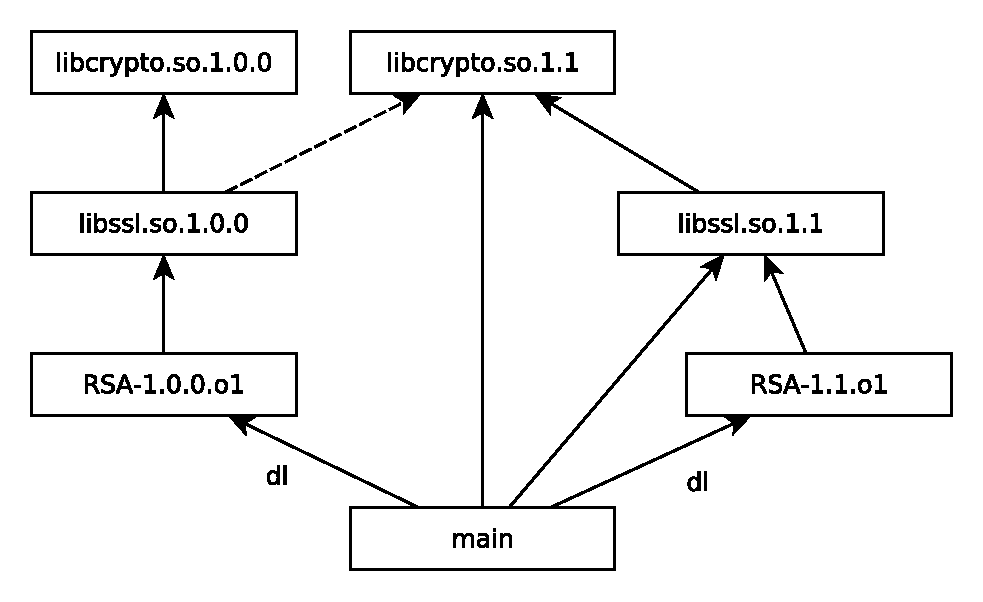
\includegraphics{figures/libssl_masking.pdf}

\caption{Schéma des dépendances entre les bibliothèques au sein d'un
  processus.  Les dépendances qui ont été liées dynamiquement durant la création
  de l'application sont représentées par une flèche avec trait plein sans
  annotation. Ceux qui représentent les chargements de bibliothèque dynamique via
  \texttt{dlopen} ont l'annotation \textit{dl}. La flèche en pointillé indique
  un masquage des symboles de la bibliothèque source par une ligne pointée.}

\label{fig:scm_masq_schema}
\end{figure}
\end{center}

%\begin{lstlisting}[frame=single]
%(c-define-type RSA* (pointer "RSA"))
%\end{lstlisting}


%Heureuse Gambit Scheme possède un interface pour lié
%une fonction C au monde Scheme.

%Une bibliothèque liant les fonctions principales de SDL au monde Scheme.


%\TODO{Fill}
% SDL / SDL2
% - Hypothèse
% - Démarche
% - Résultat
% - Petite Conclusion

% OpenSSL+RSA
% - Hypothèse
% - Démarche
% - Résultat
% - Petite Conclusion

% RNG-splitmx64/RNG-xoroshiro128+
% - Hypothèse
% - Démarche
% - Résultat
% - Petite Conclusion


\subsection{Bibliothèque JavaScript (NodeJS)}
% Démarche général
% express / sqlite3
% - Hypothèse * 2
% - Démarche/Expérimentation
% - Résultat
% - Petite Conclusion

Des tests similaires ont été effectués avec les bibliothèques JavaScript pour
montrer la coexistence de bibliothèques dans un langage interprété.

Pour effectuer des tests sur la coexistence de différente version d'une bibliothèque
JavaScript dans NodeJS, il faut tout d'abord permettre l'importation de plusieurs
versions d'une même bibliothèque. Dans NodeJS, l'importation de modules s'effectue
avec la fonction \verb|require(module-name)|. Puisque l'information de version
de la bibliothèque n'est pas fournie en paramètre à la fonction, il faut donc
utiliser une autre méthode pour forcer plusieurs versions des bibliothèques.
La configuration d'un module dans NodeJS utilise le format JSON pour spécifier
le nom, la version, les dépendances, etc.

Les dépendances sont conservées sous la forme d'un arbre, chaque module à ses dépendances directes
qui ont aussi des dépendances indirectes.  Lors de l'écriture d'un module JavaScript, il est possible
de spécifier la version de chaque dépendance dans le fichier \textit{package.json}.
\begin{verbatim}
{
  ...
  "dependencies": {
    "express": "4.16.3"
  },
  ...
}
\end{verbatim}
En utilisant cette fonctionnalité du système de module de NodeJS, deux bibliothèques \textit{wrapper}
sont écrites pour interfacer les deux versions de express. Puisque l'API public d'express n'a pas changé entre
les versions 3.21.1 et 4.16.3, il est possible de recycler le code de la bibliothèque qui encapsule une
version d'express (figure-\ref{fig:express}).
\begin{center}
\begin{figure}[ht]
    % FIXME: language=Javascript
    \begin{lstlisting}[language=C,frame=single]
const express = require('express');

function start() {
  const app = express();
  const port = Math.floor(Math.random() * 64535 + 1000);

  app.get('/', (req, res) => {
    res.send('Hello world!\n');
  });

  app.listen(port, 'localhost', () => {
    console.log('Listen on port ' + port);
  });
}
exports.start = start;
\end{lstlisting}
  \caption{Structure du module JavaScript utilisé comme proxy vers deux version
    de la bibliothèque \texttt{express}.}
  \label{fig:express}
\end{figure}
\end{center}
Le programme principal ne fait qu'importer les deux encapsulations de bibliothèque
et invoque la fonction \textit{start}.

Le résultat attendu dans cette expérience est que ces deux versions de la bibliothèque
express coexistent sans problème, sauf dans le cas où le port TCP utilisé par les deux
versions est le même. Si le port TCP est le même, c'est la bibliothèque dont la fonction
\textit{start} a été invoquée en premier qui va monopoliser le port TCP. Dans ce cas
la ressource qui inhibe la coexistence de ces modules au sein d'un même processus
est liée au \textit{socket}.

\subsection{Variables globales communes}

Les bibliothèques au sein d'une application sont chargées de façon unique.
Puisqu'il n'existe qu'une seule instance de chaque bibliothèque dans un
processus, les variables globales d'une bibliothèque sont partagées. Ces variables
composent l'état de la bibliothèque.

L'expérience définit 3 bibliothèques \texttt{B}, \texttt{C} et \texttt{D}. La bibliothèque
\texttt{D} exporte une variable globale. Les bibliothèques \texttt{B} et \texttt{C} dépendent
de \texttt{D}. Le programme principal utilise les bibliothèques \texttt{B} et \texttt{C}.
La figure~\ref{fig:libdep_experience_global_var} est une représentation graphique des dépendances
présente dans l'expérience.

\begin{figure}[ht]
  \centering
  \includegraphics[scale=0.75]{figures/libdep_experience_global_var}
  \caption{Le graphe de dépendance des bibliothèques \texttt{B}, \texttt{C} et \texttt{D}
    avec l'application \texttt{Programme}.}
  \label{fig:libdep_experience_global_var}
\end{figure}

La notation \texttt{X.Y.val} exprime une référence à la variable \texttt{val}
de \texttt{Y} à partir de la bibliothèque \texttt{X}.

Les étapes exécutées par le programme dans l'expérience sont les suivantes:
\begin{enumerate}
  \item charge les bibliothèques \texttt{B} et \texttt{C};
  \item affiche le contenu de \texttt{B.D.value} et \texttt{C.D.value};
  \item modifie le contenu de \texttt{B.D.value};
  \item affiche le contenu de \texttt{B.D.value} et \texttt{C.D.value}.
\end{enumerate}
L'expérience indique si la référence à la variable globale \texttt{value} défini
dans \texttt{D} est partagé entre les bibliothèques \texttt{B} et \texttt{C}.
Les valeurs de \texttt{B.D.value} et \texttt{C.D.value} doivent être égales à l'étape 2.
Les variables sont partagées si la condition \verb+B.D.value == C.D.value+ est vraie après
l'étape 3 de l'expérience.\\
\begin{figure}[ht]
  \centering
  \lstset{frame=single}
  \begin{mplisting}{0.5}
1- B.D.value: 0,  C.D.value: 0
2- set B.D.value 42
3- B.D.value: 42,  C.D.value: 42
\end{mplisting}
  \caption{Les résultats de l'expérience avec des bibliothèques natives du système d'exploitation sous Linux.}
  \label{fig:result_global_var_experiment}
\end{figure}

Le résultat de l'expérience de la figure~\ref{fig:result_global_var_experiment} montre
que chacune des variables globales d'une bibliothèque partagée existe qu'en une seule
instance.


% Le programme principal commence par charger les bibliothèques \texttt{B} et \texttt{C}.
% Ensuite affiche le contenu de \textit{B.D.value}
% puis modifie \textit{C.D.value} et relit \textit{B.D.value}. Le test réussi si la valeur de
% \textit{B.D.value} reste inchangée par la modification de \textit{C.D.value}. Cela implique que
% les références vers la bibliothèque D est différentes de via B et via C.

%Dans NodeJS, un module peut être installé via un dossier, une archive tarball, un dépôt de code source git ou
%directement via Npmjs. Puisqu’un module publié dans Npmjs ne peut pas être retiré facilement étant donné
%la politique liée au module (\url{https://docs.npmjs.com/cli/unpublish}).
%%L'expérience va utilisé un serveur git qui est auto-hébergé.


\section{Conclusion}
%
Ce chapitre a traité du fonctionnement de l'éditeur de lien et des
bibliothèques dynamiques. Des expériences ont été effectuées pour déterminer
les conditions sous lesquelles des bibliothèques dynamiques peuvent
coexister. Les résultats des expériences nous ont permis de déterminer
que les bibliothèques dynamiques sont en conflit lorsqu'ils exportent
les mêmes identifiants ou utilisent des ressources communes (e.g. clavier,
souris).
Nous avons aussi déterminé que l'utilisation de variables globales peut entraîner
des problèmes de coexistence entre des bibliothèques. Ils apparaissent dans
plusieurs langages de programmation interprétés. Les états globaux dans
une bibliothèque doivent être évités.
Ces conflits présents dans les bibliothèques dynamiques
du système d'exploitation peuvent être propagés par la FFI du langage
de programmation.

Le système de module que nous avons développé pour Scheme permet en principe la
coexistence de différentes versions d'un module Scheme. Cependant, si la FFI est utilisée
pour interfacer à des bibliothèques dynamiques du système d'exploitation qui
ne peuvent pas coexister cela va indirectement empêcher la coexistence des modules en
qui en dépendent. C'est un problème incontournable qu'il faut garder à l'esprit
lors de la conception des modules Scheme.


